
\chapter{Project Methodologies}\label{C:m}

\section{Project management approach}
The project methodology followed in this project was using a spiral model. This model used included requirements analysis, design, implementation, and evaluation phases. These phases  
\begin{figure}[h!]
  \centering
      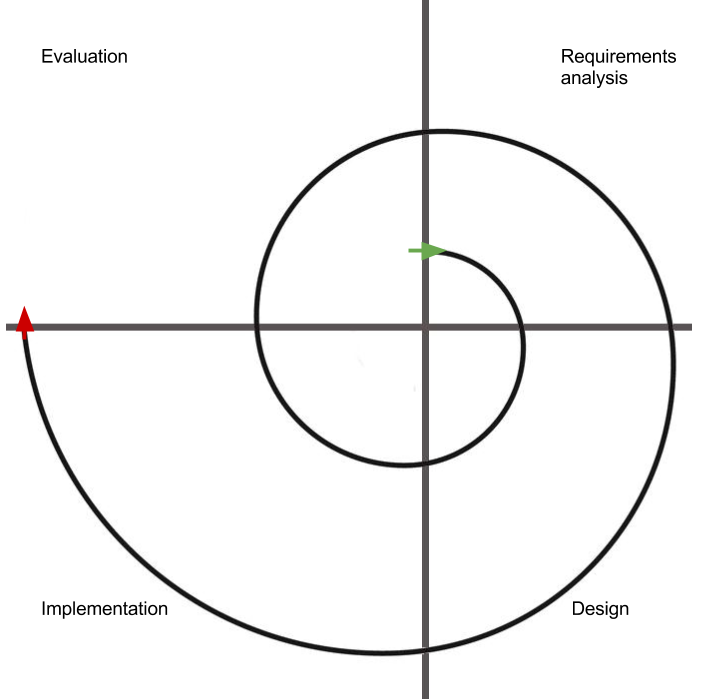
\includegraphics[width=0.8\textwidth]{images/spiral_model.png}
  \caption{Spiral process model followed}
\end{figure}
For each feature produced in the visualisation a full iteration of the spiral was completed.
\\\\
This project management technique supported the creation of a visualisation as 
\\\\
The advantages of this methodolgy over others such as stricter models such as the waterfall model or a looser agile aproach......The reason that this was effective.......
\\\\
The choice of this project management apprach meant ....
\\\\
Weekly meetings with the supervisor of the project, Dr Stuart Marshall, were used to provide guidance and 
\\\\
Using using other supporting project management techniques such as Gantt charts [APPENDIX] and work breakdown structures(WBS) [APPENDIX] allowed efficient documentation of planning and work completed in the project as well as displaying the following stages requried to complete the project.

\section{System design approach}
By choosing to expand on an already exisiting system


\section{Key difficulties encountered}
As this project builds upon a previous system much of the exisiting code and execution flow needs to be modified. This requires understanding of how the system was originally built and designed. Because this system does not have any unit or integration tests, going ahead without a comprehenive knowledge of the core functionality would be foolish.

Having a time constraint of 300 hours for this project over the course of a year meant that ...........